\chapter{Socio-economic environment}\label{ch:socio_economic_environment}

The widespread adoption of automated parking management systems is transforming urban environments and the economy, offering significant benefits while also presenting challenges. This chapter examines the socio-economic factors influencing the deployment of these systems, particularly in residential communities. It explores the potential advantages, obstacles, and financial implications of integrating this technology across urban areas.

\section{Social Impact}

Automated parking management systems have gained popularity due to their efficiency and ability to optimize space utilization, revolutionizing urban planning and mobility. Their capacity to reduce traffic congestion and improve parking availability can greatly enhance urban living conditions. For example, sensor-based systems can guide drivers to available parking spots, reducing time spent searching and lowering emissions. The project demonstrated how these systems can provide real-time occupancy data, aiding both residents and visitors in finding parking more efficiently.

In densely populated urban areas, automated parking systems facilitate better use of limited space. This capability not only improves the quality of life for residents but also contributes to more sustainable urban development by maximizing the use of available land.

However, privacy and data security remain concerns. The extensive data collection by these systems raises issues of surveillance and personal data protection, underscoring the need for clear regulations and ethical guidelines, as discussed in the regulatory framework chapter.

\section{Economic Impact}

The economic benefits of adopting automated parking management systems are substantial, with the potential to boost urban efficiency and drive innovation. For property managers and urban planners, these systems enable more efficient use of space, potentially increasing property values and reducing operational costs associated with parking management.

Despite these advantages, the costs of implementing automated parking systems (e.g., installation, training, maintenance, and upgrades) remain significant barriers for some communities and smaller property management companies. Moreover, the need for technical expertise and the risk of system failures can increase operational expenses.

\section{Environmental Impact}

Automated parking management systems can positively impact the environment by reducing traffic congestion and associated emissions. By guiding drivers directly to available spots, these systems minimize the time vehicles spend idling or circling in search of parking, contributing to lower air pollution and fuel consumption in urban areas.

Nonetheless, the environmental costs of manufacturing and disposing of electronic components must be considered. The production of sensors, cameras, and other hardware components can be resource-intensive. Sustainable design practices and proper e-waste management are necessary to mitigate these effects.

\section{Project Planning}

The project was structured into distinct phases, each with specific activities and tasks, as illustrated in \cref{fig:planning}. The timeline for these phases was planned on a weekly basis, detailing the progression of activities from initial research to final deployment. The first month and a half of the project was dedicated to understanding the problem, reviewing relevant literature, exploring the necessary tools, and configuring them for our specific needs. This initial phase, encompassing research and planning, required a significant time investment due to the complexities and documentation gaps associated with certain tools like AWS or hardware integration. The subsequent five months were focused on development of the system and the final three months to writing the final document.

\begin{figure}
    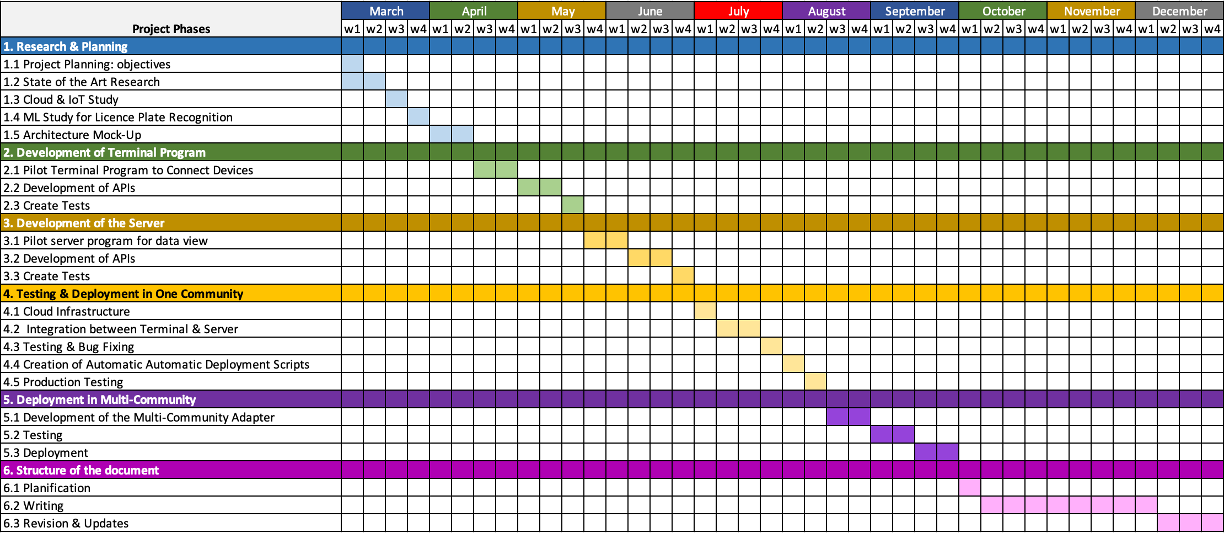
\includegraphics{planning.png}
    \caption{Gantt Chart for the Project Planning}\label{fig:planning}
\end{figure}

\section{Project Budget}

The cost of implementing automated parking management systems is a significant consideration for many communities. The analysis includes a detailed assessment of hardware components, software, maintenance, and other relevant expenses.

\cref{tab:hardware_costs_physical_components} details hardware costs for terminals, cameras, and networking equipment costs and other expenses for each community. The total cost for these physical components is estimated at 621 \euro\ per community. However, it is worth noting that for this project, 10 different communiteis have been installed totaling to 6210 \euro\ for the physical components. Moreover, in \cref{tab:costs_software_components} the cost of the software components are included totaling to 30 \euro. Moreover, the human costs associated to this project, refer to \cref{tab:human_costs}, amount to 13900 \euro.

For this project, the total cost would amount to 20140 \euro, which includes the necessary hardware and software for a typical residential community and the human labor costs. However, it's important to note that this does not account for installation and long-term maintenance costs or potential upgrades, which are essential for the system's longevity and effectiveness.

In conclusion, while automated parking management systems hold significant promise for urban areas and residential communities, careful consideration of social, economic, and environmental factors is essential. Addressing these challenges with appropriate regulations and sustainable practices will maximize their potential benefits in creating more livable and efficient urban spaces.

\begin{table}[H]
	\begin{tabular}{ l l r r }
		\toprule
		\textbf{Item}               & \textbf{Model}                                & \textbf{Quantity} & \textbf{Cost (\euro)} \\
		\midrule
		Edge Computer               & NVIDIA Jetson Nano \autocite{reComputerJ1010} & 1                 & 220                   \\
		Cameras                     & Reolink RLC-811A \autocite{ReolinkRLC811A}    & 2                 & 166                   \\
		Router                      & TP-Link AC1200 \autocite{TPLinkArcherMR600}   & 1                 & 85                    \\
		Reles                       &                                               & 1                 & 10                    \\
		Ethernet Cables             & Cat 6 30 meters                               & 1                 & 20                    \\
		4G SIM Card                 & Orange Prepaid SIM Card (1 month)             & 1                 & 10                    \\
		Boxes, power supplies, etc. &                                               & 1                 & 100                   \\
		\midrule
		\textbf{Total}              &                                               &                   & 621                   \\
		\bottomrule
	\end{tabular}
	\caption{Hardware costs for the physical components for one community.}\label{tab:hardware_costs_physical_components}
\end{table}

\begin{table}[H]
	\begin{tabular}{ l l l r }
		\toprule
		\textbf{Item}  & \textbf{Model}                           & \textbf{Quantity} & \textbf{Cost (\euro)} \\
		\midrule
		Server         & Amazon Web Services Deployment (1 month) & 1                 & 30                    \\
		\midrule
		\textbf{Total} &                                          &                   & 30                    \\
		\bottomrule
	\end{tabular}
	\caption{Costs for the software components and maintenance.}\label{tab:costs_software_components}
\end{table}

\begin{table}[H]
    \begin{tabular}{ l l l r }
        \toprule
		\textbf{Item}  & \textbf{Model}                           & \textbf{Quantity} & \textbf{Cost (\euro)} \\
        \midrule
        Personal Computer & Macbook Air & 1 & 1600  \\
        Junior Engineer Hours & 15 \euro/h & 500 & 7500 \\
        Senior Engineer Hours & 60 \euro/h & 40 & 2400 \\
        Electricity, labs, climate control, management, etc. & & & 2040 \\
        \midrule
        \textbf{Total} & & & 13900 \\
        \bottomrule
    \end{tabular}
    \caption{Human costs.}\label{tab:human_costs}
\end{table}
